\section{Level Set Method}
\label{levelSetChap}
\subsection{Introduction}
Surfaces that evolves over time can be difficult to represent. Taking the surface in figure \ref{interface} as an example, assume that the red surface is heat and the arrows on the interface as the direction of its movement, which is normal to the interface itself. One way to represent the propagation of this interface is by the function $y = f(x,t)$, where $t$ represents time and $x,y$ are coordinates. The problem with this representation is that it cannot represent every concievable shape of the interface. If for instance the shape
of the inerface has more y coordinates for a particular x coordinate (which is true for all closed interfaces), the intercane cannot be correctly represented using this notion.
\begin{figure}[h!]
\centering
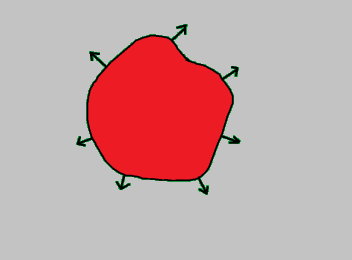
\includegraphics[width=.5\textwidth]{backgroundTheory/levelset/interface}
\caption{Interface of a moving surface.}
\label{interface}
\end{figure}
A better alternative is to use a parametric equation. The problem mentioned above would then be solved because the interface would only depend on the time variable t. But parametric representation of evolving interfaces have its own difficulties. When a surface evolves, the model have to be reparemeterized, which, due to the computional overhead (especially in 3D) add limitations to what kind of shapes a parameterical model can represent effectively. Topological changes, such as splitting or merging parts during the propagation is difficult to represent using parametric models. Sharp corners, distant edges blending together and the complexity of representing boundaries in higher dimensions are some other reasons why an evolving surface is difficult to represent parametrically. A simple example is shown in figure \ref{problematicEvo}, the two interfaces have to be represented as a single parametric function when merging and as two seperate againg when they split, and some sort of collison detection must be used to discover when the interfaces merge/split.
\begin{figure}[h!]
\centering
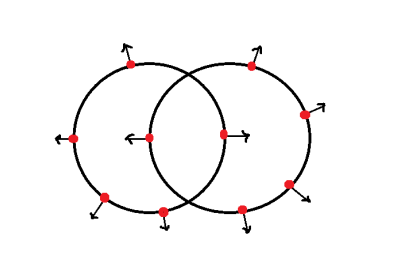
\includegraphics[width=.5\textwidth]{backgroundTheory/levelset/twoCircles}
\caption{Interface evolution difficult to represent parametrically.}
\label{problematicEvo}
\end{figure}

As a solution to all the problems mentioned above Osher and Sethian introduced the level set method in 1988 in \cite{osher88}. The main idea behind the level set method is to represent the interface of a surface implicitly by using a higher dimensional function. Adding an extra dimension simplifies the problems mentioned above significantly. This higher dimension function is called the level set function, and a 2D interface (a curve) is represented by the 3D level set function
\begin{equation}
\phi(x, y, t) 
\end{equation}
where the additional dimension \(t\) represents time. Similarly any 3D or higher level function can be represented by a level set function by adding one dimension. At a given time step, the evolving surface/model can be represented as a closed curve by the boundary of the level set at that time step. This representation of the model is called the zero level set and is defined as the set of points where the level set is zero:
\begin{equation}
\Gamma(x, y, t) = \{\phi(x, y, t) = 0\}. 
\end{equation}
The initial curve is at the xy-plane, that is, at \(\phi(x,y,0)\). As an example, figure \ref{levelsetEx}a depicts a circle with arrows pointing in the direction it is evolving, and figure \ref{levelsetEx}b is the cone that represents the corresponding level set function with the start-position in red.

\begin{figure}[h!]
\centering
\begin{minipage}{.4\textwidth}
\begin{tabular}{c}
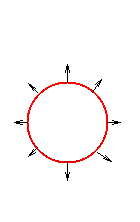
\includegraphics[height=.3\textheight]{backgroundTheory/levelset/f1a} \\
(a)
\end{tabular}
\end{minipage}
\begin{minipage}{.4\textwidth}
\begin{tabular}{c}
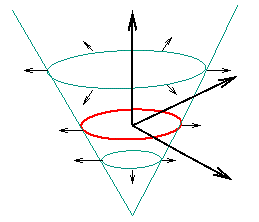
\includegraphics[height=.3\textheight]{backgroundTheory/levelset/f1b} \\
(b)
\end{tabular}
\end{minipage}
\caption{(a): Circle with arrows pointing in direction of movement, (b): Corresponding level set function}
\label{levelsetEx}
\end{figure}

Assuming that the zero level set moves in a direction normal to the speed F, then \(\phi\) satisfies the level set equation
\begin{equation}
\frac{\partial \phi}{\partial t} = |\nabla \phi|F
\label{levelSetEq}
\end{equation}
which is used to update the level set at each time step (iteration). Here \(|\nabla \phi|\) represents the gradient of \(\phi\), and the speed function F describes how each point in the boundary of the surface evolves. The level set method is applied in many different contexts, such as image processing, fluid dynamics and other simulations, and the speed function F depends on the type of problem being considered. 

An often used speed function for image segmentation that combines a data term and the mean curvature of the surface is \cite{cates03,lefohn04}
\begin{equation}
F = \alpha D(I) + (1-\alpha) \nabla \frac{\nabla \phi}{|\nabla \phi|}
\end{equation} 
where \(\nabla \cdot (\nabla \phi / |\nabla \phi|)\) is the normal vector that represents the mean curvature term which keeps the level set function smooth. \(D(I)\) is the data function that forces the model towards desirable features in the input data. The free weighting parameter \(\alpha \in{[0,1]}\) controls the level of smoothness, and I is the input data (the image to be segmented). The smoothing term \(\alpha\) restricts how much the curve can bend and thus alleviates the effect of noise in the data, preventing the model from leaking into unwanted areas\cite{lefohn04}. This is one of the big advantages the level set method has over classical flood fill, region grow and similar algorithms, which does not have a constraint on the smoothness of the curve.

A simple data function for any point (pixel, voxel) based solely on the input intensity I at that point\cite{cates03,lefohn04} is:
\begin{equation}
D(I) = \epsilon - |I - T|
\end{equation} 
Here \(T\) is the central intensity value of the region to be segmented, and \(\epsilon\) is the deviation around \(T\) that should also considered to be inside the region. This makes the model expand if the intensity of the points are within the region \(T \pm \epsilon\), and contract otherwise. The data function is gradual, thus the effects of \(D(I)\) diminish as the model approaches the boundaries of regions with gray-scale levels within the \(T \pm \epsilon\) range \cite{lefohn04}. This results in the model expanding faster with higher values of \(\epsilon\) and slower with lower values. 

The level set algorithm is initialized by placing a set of seed points that represents a part inside the region to be segmented. These seed points are represented by a binary mask of the same size as the image to be segmented. This mask is used to compute the signed distance function which \(\phi\) will be initialized to. 

\subsection{Signed Distance Transform}
A distance function \(D: \mathbb{R}^3 \rightarrow \mathbb{R}\) for a set S is defined as 
\begin{equation}
D(r,S) = min(r-S) \quad for \ all \ r \in{\mathbb{R}^3}
\end{equation}
If a binary image have one or more objects, a distance function can be used to assign a value for every pixel (or voxel in 3D) that represents the minimum distance from that pixel to the closest pixel in the boundary of the object(s). That is, the pixels in the boundary of an object are zero valued, and all other pixels represent the distance to the boundary as a value. Using a distance transform was the idea of how to initialize \(\phi\) in \cite{osher88}, where it was initialized as \(\phi = 1 \pm D^2\). But in \cite{mulder92} it was showed that initializing \(\phi\) to a signed distance function gives more accurate results. Signed distance transforms (SDT) assign for each pixel a value with a positive or negative sign that depend on whether the pixel is inside or outside the object. The values are usually set to be negative for pixels that are inside an object, and positive for those outside. The pixels of the model, which represents the boundary (the zero level set), have values 0. A binary image containing an object is shown in figure \ref{SDT}a (the numbers in this image represent intensity values). Figure \ref{SDT}b is the signed distance transform of \ref{SDT}a where city-block (manhattan) distance have been used, and figure \ref{SDT}c is the signed Euclidean distance transform (SEDT).

\begin{figure}[h!]
\centering
\begin{minipage}{.45\textwidth}
\begin{tabular}{c}
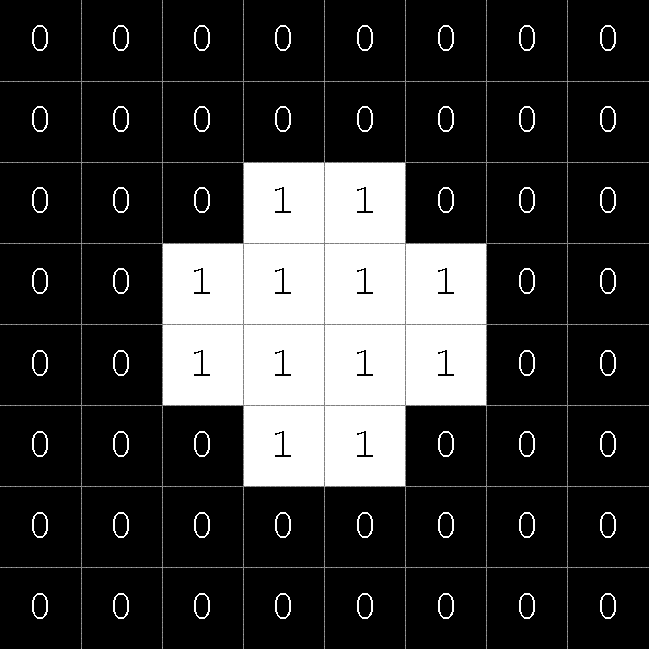
\includegraphics[width=.9\textwidth]{backgroundTheory/levelset/orgNew} \\
(a)
\end{tabular}
\end{minipage}
\begin{minipage}{.45\textwidth}
\begin{tabular}{c}
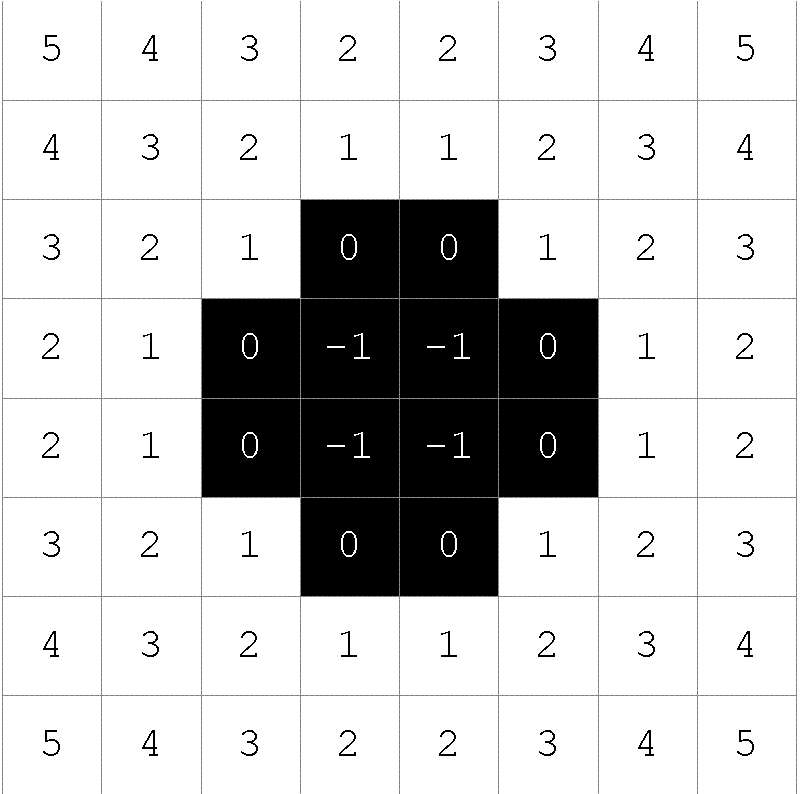
\includegraphics[width=.9\textwidth]{backgroundTheory/levelset/manhattan} \\
(b)
\end{tabular}
\end{minipage}
\\
\begin{tabular}{c}
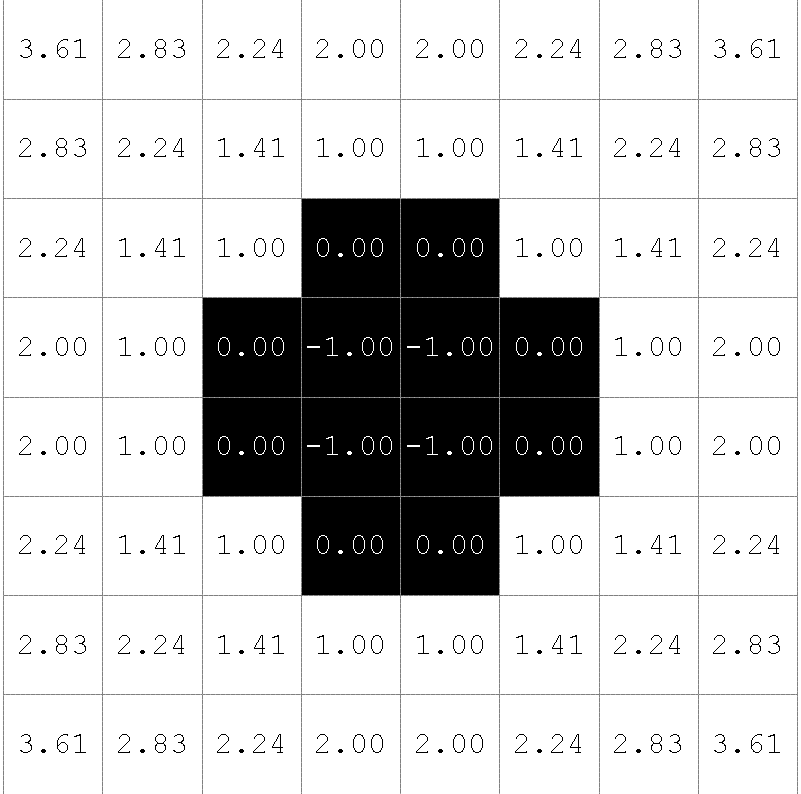
\includegraphics[width=.5\textwidth]{backgroundTheory/levelset/euclidean} \\
(c)
\end{tabular}
\caption{(a): Binary image, (b): SDT based on city-block distance, (c): SDT based on euclidean distance}
\label{SDT}
\end{figure}

As can be seen from the figures above, using different kind of functions for the SDT can result in different distances. These differences effects the accuracy of the level set function, which may leads to different end-results of the segmentation, hence, the function used to represent the distance have to be carfully chosen. However, sometimes a less accurate SDT have to be used as a tradeoff for faster computation time.

%\subsection{Sparse Field}
%The narrow band  method assumes that the computation of the SDT is so slow that it cannot be computed for every iteration (time step). The sparse field method introduced in \cite{whitaker89} uses a fast approximation of the distance transform that makes it feasible to compute the neighborhood of the level set model for each iteration. In the sparse field method the idea of using a thin band is taken to the extreme by working on a band that is only one point wide. The points adjacent to the level set are called active points, and all of them together are referred to as the active set. At each iteration only a thin layer of points near the active set are visited and updated. Using only the active points to compute the derivatives would not give sufficient accuracy. Because of this, the method extends out from the active points in small layers to create a neighborhood that is precisely the width needed to calculate the derivatives needed. 

%Several advantages to this approach are mentioned in \cite{whitaker89}. No more than the precise number of calculations to find the next position of the zero level set surface is used. The number of points being computed is so small that a linked-list can be used to keep track of them. This also results in that only those points whose values control the position of the zero level set surface are visited at each iteration. A disadvantage of the narrow band method is that the stability at the boundaries of the band have to be maintained (e.g. by smoothing) since some points are undergoing the evolution while other neighbouring points remain fixed. The sparse field method avoid this by not letting any point entering or leaving the active set affecting its value. A point enters the active set if it is adjacent to the model. As the model evolves, points in the active set that are no longer adjacent to the model are removed from the active set. This is done by defining the neighborhoods of the active set in layers and keeping the values of points entering or leaving the active set unchanged. A layer is a set of pixels represented as \(L_{i}\) where \(i\) is the city-block distance from the active set. The layer \(L_{0}\) represents the active set, and \(L_{\pm 1}\) reprsents pixels adjacent to the active set on both sides. Using linked lists to represents the layers and arrays (matrices) to represent distance values makes the algorithm very efficient. The exact steps of the sparse field algorithm can be found in \cite{whitaker89}.

%The sparse field algorithm is based on an important approximation, it assumes that points adjacent to the active points undergoes the same change in value as their nearby active set neighbors. But despite this, the errors introduced by the sparse field algorithm are no worse than many other level set algorithms. Since only those grid points whose values are changing (the active points and their neighbors) are visited at each time step the growth computation time is \(d^{n-1}\), where d is the number of pixels in along one dimension of the image. This is the same as for parameterized models where the computation times increase with the resolution of the domain, rather than the range.

\subsection{Discretization by upwinding and difference of normals}
\label{upwinding}
To use the level set method in image processing it have to be discretized, but simple forward finite difference schemes cannot be used because such schemes tends to overshoot and are unstable. To overcome this problem the up-winding scheme was proposed in \cite{osher88}. To avoid the overshooting problems associated with forward finite differences the up-winding scheme uses one-sided derivatives that looks in the up-wind direction of the moving interface. Let \(\phi^n\) and \(F^n\) represent the values of \(\phi\) and \(F\) at some point in time \(t^n\). The updating process consist of finding new values for \(\phi\) at each point after a time interval \(\Delta t\). The forward Euler method is used to get a first-order accurate method for the time discretization of equation \ref{levelSetEq}, given by (from \cite{osher02})
\begin{equation}
\frac{\phi^{n+1}-\phi^n}{\Delta t} + F^n \cdot \nabla \phi^n = 0
\label{discEq}
\end{equation}
where \(\phi^{n+1}\) is \(\phi\) at time \(t^{n+1} = t^n + \Delta t\), and \(\nabla \phi^n\) is the gradient at time \(t^n\). This equation is expanded as follows (for three dimensions):
\begin{equation}
\frac{\phi^{n+1}-\phi^n}{\Delta t} + u^n \phi_x^n + v^n \phi_y^n + w^n \phi_z^n= 0,
\label{discEqExpanded}
\end{equation}
where the techniques used to approximate the \(u^n \phi_x^n\), \(v^n \phi_y^n \) and \(w^n \phi_z^n\) terms can be applied independently in a dimension-by-dimension manner \cite{osher02}. When looking at only one dimension (for simplicity), the sign of \(u^n\) would indicate whether the values of \(\phi\) are moving to the right or to the left. The value \(u^n\) can be spatially varying, hence by looking at only one point \(x_i\) in addition to only look at one dimension, equation \ref{discEqExpanded} can be written as
\begin{equation}
\frac{\phi_i^{n+1}-\phi_i^n}{\Delta t} + u_i^n (\phi_x)_i^n = 0,
\label{discEq1DPoint}
\end{equation}  
where \((\phi_x)_i^n\) denotes the spatial derivative of \(\phi\) at point \(x_i\) at time \(t^n\). The values of \(\phi\) are moving from left to right if \(u_i > 0\), thus the points to the left for \(x_i\) are used to determine the value of \(\phi\) at point \(x_i\) for the the next time step. Similarly, if \(u_i < 0\) the movement is from right to left, and the points to the right of \(x_i\) are used. As a result, \(\phi_x\) is approximated by the derivative function \(D_x^+\) when \(u_i < 0\) and \(D_x^-\) when \(u_i > 0\). When \(u_i = 0\) the term \(u_i(\phi_x)_i\) equals zero, and approximation is not needed. Extending this to three dimensions, the derivatives used to update the level set equation are 
\begin{equation*}
\nonumber D_x = \frac{\phi_{i+1,j,k} - \phi_{i-1,j,k}}{2} \quad D_y = \frac{\phi_{i,j+1,k}-\phi_{i,j-1,k}}{2} \quad D_z = \frac{\phi_{i,j,k+1}-\phi_{i,j,k-1}}{2} 
\end{equation*}
\begin{equation*}
\nonumber D_x^+ = \phi_{i+1,j,k} - \phi_{i,j,k} \quad D_y^+ = \phi_{i,j+1,k} - \phi_{i,j,k} \quad D_z^+ = \phi_{i,j,k+1} - \phi_{i,j,k} 
\end{equation*}
\begin{equation*} 
D_x^- = \phi_{i,j,k} - \phi_{i-1,j,k} \quad D_y^+ = \phi_{i,j,k} - \phi_{i,j-1,k} \quad D_z^+ = \phi_{i,j,k} - \phi_{i,j,k-1}
\end{equation*}
\begin{equation}
\quad %to get a reference number below the equations
\end{equation}
which is taken from the appendix of \cite{lefohn04}. This is a \textit{consistent} finite difference approximation to the level set equation in \ref{levelSetEq}, because the approximation error converges to zero as \(\Delta t \rightarrow 0\) and \(\Delta x \rightarrow 0\) \cite{osher02}. In addition to being consistent, it also have to be \textit{stable} in order to get the correct solution. Stability guarantees that small errors in the approximations are not amplified over time. The stability can be enforced using the  Courant-Friedreichs-Lewy (CLF) condition which says that the numerical wave speed \(\frac{\Delta x}{\Delta t}\) must be greater than the physical wave speed \(|u|\),
\begin{equation}
\Delta t = \frac{\Delta x}{max\{|u|\}},
\end{equation}
where \(max\{|u|\}\) is the largest value of \(|u|\) on the model.

The gradient \(\nabla \phi\) is approximated to either \(\nabla \phi_{max}\) or \(\nabla \phi_{min}\) depending on whether the speed function for a given point \(F_{i,j,k}\) is positive or negative, 
\begin{equation}
\nabla \phi = \left\{
\begin{array}{l l}
||\nabla \phi_{max}||_2 & F_{i,j,k}>0 \\
||\nabla \phi_{min}||_2 & F_{i,j,k}<0
\end{array} \right.
\end{equation}
where \(\nabla \phi_{max}\) and \(\nabla \phi_{min}\) is given by (from \cite{lefohn04})
\begin{equation}
\nabla \phi_{max} = \begin{bmatrix}
\: \sqrt{max(D_x^+,0)^2 + max(-D_x^-,0)^2} \: \\[1.5em]
\: \sqrt{max(D_y^+,0)^2 + max(-D_y^-,0)^2} \: \\[1.5em]
\: \sqrt{max(D_z^+,0)^2 + max(-D_z^-,0)^2} \: 
\end{bmatrix} 
\end{equation}
\newline
\begin{equation}
\nabla \phi_{min} = \begin{bmatrix}
\: \sqrt{min(D_x^+,0)^2 + min(-D_x^-,0)^2} \: \\[1.5em]
\: \sqrt{min(D_y^+,0)^2 + min(-D_y^-,0)^2} \: \\[1.5em]
\: \sqrt{min(D_z^+,0)^2 + min(-D_z^-,0)^2} \: 
\end{bmatrix} 
\end{equation}

The curvature term \(\nabla \cdot (\nabla \phi / |\nabla \phi|)\) of the speed function \(F\) is discretized using the difference of normals method. The second order derivatives are computed first:
\begin{equation*}
D_x^{+y} = (\phi_{i+1,j+1,k} - \phi_{i-1,j+1,k})/2 \quad D_x^{-y} = (\phi_{i+1,j-1,k} - \phi_{i-1,j-1,k})/2 
\end{equation*}
\begin{equation*}
D_x^{+z} = (\phi_{i+1,j,k+1} - \phi_{i-1,j,k+1})/2 \quad D_x^{-z} = (\phi_{i+1,j,k-1} - \phi_{i-1,j,k-1})/2 
\end{equation*}
\begin{equation*}
D_y^{+x} = (\phi_{i+1,j+1,k} - \phi_{i+1,j-1,k})/2 \quad D_y^{-x} = (\phi_{i-1,j+1,k} - \phi_{i-1,j-1,k})/2 
\end{equation*}
\begin{equation*}
D_y^{+z} = (\phi_{i,j+1,k+1} - \phi_{i,j-1,k+1})/2 \quad D_y^{-z} = (\phi_{i,j+1,k-1} - \phi_{i,j-1,k-1})/2 
\end{equation*}
\begin{equation*}
D_z^{+x} = (\phi_{i+1,j,k+1} - \phi_{i+1,j,k-1})/2 \quad D_z^{-x} = (\phi_{i-1,j,k+1} - \phi_{i-1,j,k-1})/2 
\end{equation*}
\begin{equation*}
D_z^{+y} = (\phi_{i,j+1,k+1} - \phi_{i,j+1,k-1})/2 \quad D_z^{-y} = (\phi_{i,j-1,k+1} - \phi_{i,j-1,k-1})/2 
\end{equation*}
\begin{equation}
\quad %to get a reference number below the equations
\end{equation}
Then these derivatives are used to compute the normals \(n^+\) and \(n^-\) in equation \ref{normals}, which is used to compute the mean curvature \(H\) in equation \ref{meanCurvature} taken from \cite{lefohn04}.
\begin{equation*}
n^+ = \begin{bmatrix}
\: \frac{D_x^+}{\sqrt{(D_x^+)^2 + (\frac{D_y^{+x}+D_y}{2})^2 + (\frac{D_z^{+x}+D_z}{2})^2}} \: \\[2.5em]
\: \frac{D_y^+}{\sqrt{(D_y^+)^2 + (\frac{D_x^{+y}+D_x}{2})^2 + (\frac{D_z^{+y}+D_z}{2})^2}} \: \\[2.5em]
\: \frac{D_z^+}{\sqrt{(D_z^+)^2 + (\frac{D_x^{+z}+D_x}{2})^2 + (\frac{D_y^{+z}+D_y}{2})^2}} \:
\end{bmatrix} 
\end{equation*}
\begin{equation}
n^- = \begin{bmatrix}
\: \frac{D_x^-}{\sqrt{(D_x^-)^2 + (\frac{D_y^{-x}+D_y}{2})^2 + (\frac{D_z^{-x}+D_z}{2})^2}} \: \\[2.5em]
\: \frac{D_y^-}{\sqrt{(D_y^-)^2 + (\frac{D_x^{-y}+D_x}{2})^2 + (\frac{D_z^{-y}+D_z}{2})^2}} \: \\[2.5em]
\: \frac{D_z^-}{\sqrt{(D_z^-)^2 + (\frac{D_x^{-z}+D_x}{2})^2 + (\frac{D_y^{-z}+D_y}{2})^2}} \:
\end{bmatrix} 
\label{normals}
\end{equation}

\begin{equation}
H = \frac{1}{2}\nabla \cdot \frac{\nabla \phi}{|\nabla \phi|} = \frac{1}{2}[(n_x^+ - n_x^-) + (n_y^+ - n_y^-) + (n_z^+ - n_z^-)]
\label{meanCurvature}
\end{equation}

Finally, the level set equation is updated as
\begin{equation}
\phi(t + \Delta t) = \phi(t) + \Delta tF|\nabla \phi|.
\end{equation}